% Étude de cas
\begin{slide}[Un modèle dynamique adéquat est disponible\\
			  pour simuler correctement les PàCCV]

\node [anchor=base west, visible on=<1>] (text) at (t5cl cs:0,4) {
	\begin{minipage}[b]{\dimexpr2\colvsep+4\quanta}\raggedright
		\emph{Exemple}\\[2\baselineskip]
		Profil de consommation\\d'une unité de résidence typique,\\~\\
		avec un pas de temp $ \Delta t = \SI{1}{\minute} $
	\end{minipage}};

\node [anchor=south east, visible on=<1>] at (p5cr cs:4,3)
	{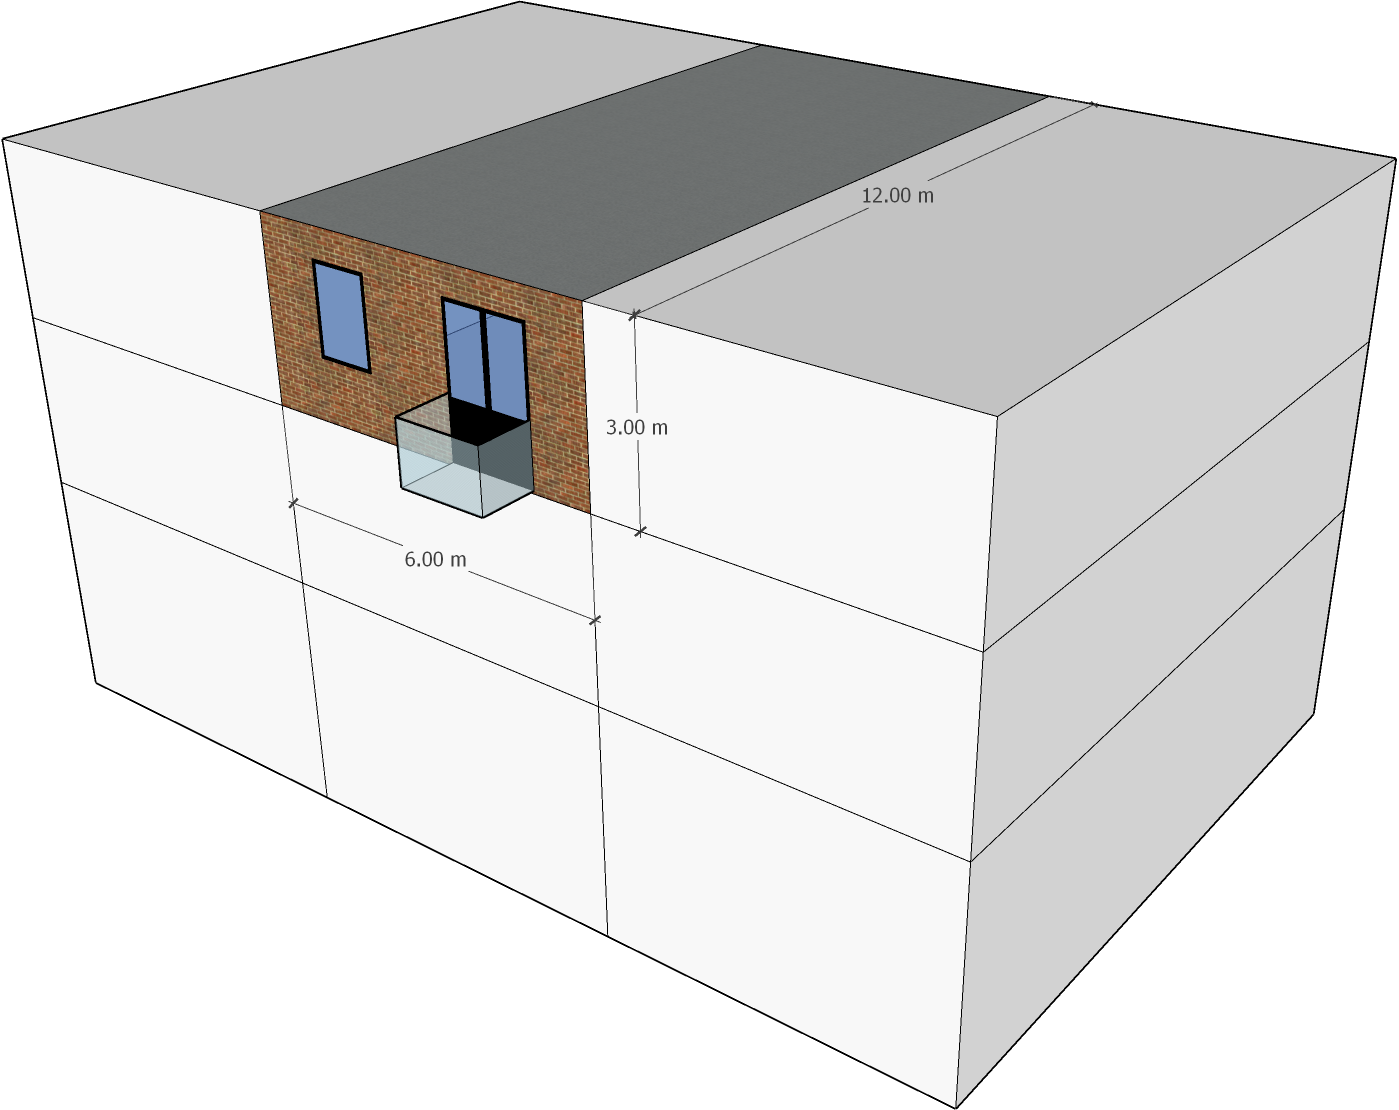
\includegraphics[height=9\baselineskip]{pictures/plex-unit}};


% cooling results
\begin{groupplot}[group style={group size=1 by 3},
				  width=3\colvsep,
				  height=3\baselineskip,
				  xmin=0, xmax=48,
				  clip=false,
				  plot options,]

\nextgroupplot[
	axis x line=none,
	ymin=11.9, ymax=31.9,
	ytick={11.9, 31.9},
	yticklabels={11.9, \SI{31.9}{\celsius}},
	at={(p5cl cs:1,11)},
	anchor=south west,
	visible on=<2>]
\addplot[thick, col] table[x=time, y=TdbAmb] {data/case-study-cool.tsv};
\node[col, font=\footnotesize] at (axis cs:38,25) {\To};

\nextgroupplot[
	axis x line=none,
	ymin=14.898, ymax=26,
	ytick={14.9, 26},
	yticklabels={14.9, \SI{26}{\celsius}},
	at={(p5cl cs:1,7)},
	anchor=south west,
	visible on=<2>]
\addplot [gray!50] coordinates{(0,26) (48,26)};
\addplot [thick, gray] table[x=time, y=TdbSupply]
	{data/case-study-cool.tsv};
\addplot [thick,  col] table[x=time, y=TdbRoom] {data/case-study-cool.tsv};
\node [col, font=\footnotesize] at (axis cs:38,24) {\Tr};
\node [gray, font=\footnotesize] at (axis cs:38,16) {\Ts};


\nextgroupplot[
	xtick={0, 12, 17, 24, 31.25, 48},
	xticklabels={0:00, 12:00, \phantom{PM }5 PM, 0:00,
				 \phantom{AM }7:15 AM, 0:00},
	xticklabel style={name=ticklabel\ticknum},
	ymin=0, ymax=2.339,
	ytick={0, 1.1, 2.339},
	yticklabels={0, 1.1, \SI{2.3}{\kilo\watt}},
	at={(p5cl cs:1,3)},
	anchor=south west,
	visible on=<2>]
\addplot [thick, gray] table [x=time, y=QCoolSen]
	{data/case-study-cool.tsv};
\addplot [thick] table [x=time, y=PTot] {data/case-study-cool.tsv};
\addplot [thick, col] table [x=time, y=QCoolLat]
	{data/case-study-cool.tsv};
\node [gray, font=\footnotesize] at (axis cs:38,2) {\Qcs};
\node [col, font=\footnotesize] at (axis cs:38,0.8) {\Qcl};
\node [font=\footnotesize] at (axis cs:38,-.2) {\Pel};

\node [gray, anchor=west, yshift=-\baselineskip, font=\scriptsize] (day1)
	at (ticklabel0.west) {June 30, 2017};
\node [gray, anchor=west, yshift=-\baselineskip, font=\scriptsize]
	at (ticklabel3.west) {July 01, 2017};
\node [left, font=\scriptsize, inner sep=4\quanta]
	at (ticklabel0.west) {$t$};
\node [left, font=\scriptsize, inner sep=4\quanta] at (day1.west) {day};

\end{groupplot}



% heating results
\begin{groupplot}[group style={group size=1 by 3},
				  width=3\colvsep,
				  height=3\baselineskip,
				  xmin=0, xmax=48,
				  clip=false,
				  plot options,]

\nextgroupplot[
	axis x line=none,
	ymin=-17.9, ymax=7.771,
	ytick={-17.9, 7.771},
	yticklabels={\num{-17.9}, \SI{7.8}{\celsius}},
	at={(p5cl cs:1,11)}, anchor=south west,
	visible on=<3>]
\addplot[thick, col] table[x=time, y=TdbAmb] {data/case-study-heat.tsv};
\node[col, font=\footnotesize] at (axis cs:5,-1) {\To};

\nextgroupplot[
	axis x line=none,
	ymin=22, ymax=41.973,
	ytick={22, 41.973},
	yticklabels={22, \SI{42}{\celsius}},
	at={(p5cl cs:1,7)}, anchor=south west,
	visible on=<3>]
\addplot [gray!50] coordinates{(0,22) (48,22)};
\addplot [thick, gray] table[x=time, y=TdbSupply]
	{data/case-study-heat.tsv};
\addplot [thick,  col] table[x=time, y=TdbRoom] {data/case-study-heat.tsv};
\node [col, font=\footnotesize] at (axis cs:5,18) {\Tr};
\node [gray, font=\footnotesize] at (axis cs:5,32) {\Ts};


\nextgroupplot[
	xtick={0, 12, 20, 24, 36, 48},
	xticklabels={0:00, 12:00, 8 PM, 0:00, 12:00, 0:00},
	xticklabel style={name=ticklabel\ticknum},
	ymin=0, ymax=4.23,
	ytick={0, 4.23},
	yticklabels={0, \SI{4.2}{\kilo\watt}},
	at={(p5cl cs:1,3)}, anchor=south west,
	visible on=<3>]
\addplot [thick, gray] table [x=time, y=QHeat] {data/case-study-heat.tsv};
\addplot [thick, col] table [x=time, y=PTot] {data/case-study-heat.tsv};
\node[gray, font=\footnotesize] at (axis cs:5,2.1) {\Qh};
\node[col, font=\footnotesize] at (axis cs:5,-.6) {\Pel};

\node [gray, anchor=west, yshift=-\baselineskip, font=\scriptsize] (day1)
	at (ticklabel0.west) {Feb 10, 2017};
\node [gray, anchor=west, yshift=-\baselineskip, font=\scriptsize]
	at (ticklabel3.west) {Feb 11, 2017};
\node [left, font=\scriptsize, inner sep=4\quanta]
	at (ticklabel0.west) {$t$};
\node [left, font=\scriptsize, inner sep=4\quanta] at (day1.west) {day};

\end{groupplot}




% defrost detail
\begin{groupplot}[group style={group size=1 by 3},
				  width=3\colvsep,
				  height=3\baselineskip,
				  xmin=0, xmax=3,
				  clip=false,
				  plot options,]

\nextgroupplot[
	axis x line=none,
	ymin=-20, ymax=-18.4,
	ytick={-20, -18.4},
	yticklabels={\num{-20}, \SI{-18.4}{\celsius}},
	at={(p5cl cs:1,11)}, anchor=south west,
	visible on=<4>]
\addplot[thick, col] table[x=time, y=TdbAmb]
	{data/case-study-heat-detail.tsv};
\node[col, font=\footnotesize] at (axis cs:0.17,-19.4) {\To};

\nextgroupplot[
	axis x line=none,
	ymin=21.4, ymax=22.4,
	ytick={21.4, 22, 22.4},
	yticklabels={21.4, 22, \SI{22.4}{\celsius}},
	at={(p5cl cs:1,7)}, anchor=south west,
	visible on=<4>]
\addplot [gray!50] coordinates{(0,22) (3,22)};
\addplot [thick,  col] table[x=time, y=TdbRoom]
	{data/case-study-heat-detail.tsv};
\node [col, font=\footnotesize] at (axis cs:0.17,21.6) {\Tr};


\nextgroupplot[
	xtick={0, 3},
	xticklabels={7:00, 10:00},
	xticklabel style={name=ticklabel\ticknum},
	ymin=0, ymax=4.5,
	ytick={0, 3.228, 4.5},
	yticklabels={0, 3.2, \SI{4.5}{\kilo\watt}},
	at={(p5cl cs:1,3)}, anchor=south west,
	visible on=<4>]
\addplot [thick, gray] table [x=time, y=QHeat]
	{data/case-study-heat-detail.tsv};
\addplot [thick, col] table [x=time, y=PTot]
	{data/case-study-heat-detail.tsv};
\node[gray, font=\footnotesize] at (axis cs:0.17,5.2) {\Qh};
\node[col, font=\footnotesize] at (axis cs:0.17,2.4) {\Pel};

\node [gray, anchor=west, yshift=-\baselineskip, font=\scriptsize] (day1)
	at (ticklabel0.west) {Jan 12, 2017};
\node [left, font=\scriptsize, inner sep=4\quanta]
	at (ticklabel0.west) {$t$};
\node [left, font=\scriptsize, inner sep=4\quanta] at (day1.west) {day};

\end{groupplot}


\end{slide}





% Travaux futurs
\begin{slide}[Certains aspects du modèle\\
			  peuvent encore être améliorés]

\node [anchor=base west] at (t5cr cs:1,2){
	\begin{minipage}[b]{2.2\colvsep}\raggedright
	\begin{listed}
		\item Correction qui dépend du débit
		\item<2-> Mode pour des simulations\\à pas de temps élevés
		\item<3-> Influence de l'humidité\\sur la capacité totale
		\item<4-> Étendre les valeurs de \Qc\\à des basses températures
		\item<5-> Tests avec la fréquence du compresseur imposée
	\end{listed}
	\end{minipage}};
	
\end{slide}
